% !TEX root = ../main.tex

\section{Examples and data analysis} \label{sec:analysis}

In this section, we provide examples and use-cases on the dataset. Code to reproduce our examples is available online, in the \texttt{examples} folder.

\subsection{Summary statistics}

First, we start by providing some summary statistics. 

\subsubsection{The roster file}
The file \texttt{roster.csv} contains information about $N=35{,}430$ CPD officers. For each officer --- identified by a Unique Identifier (``uid''), \texttt{roster.csv} provides, among other covariates, the officer's name, gender, race, birthyear, appointment and resignation dates. It is straightforward  to use the data to generate summary statistics, e.g., using appointment and resignation dates to understand the number of appointments, retirements as well as active officers over the years of  (\Cref{fig:history}). We report in \Cref{tab:stats} some 
\begin{figure}[h] 
	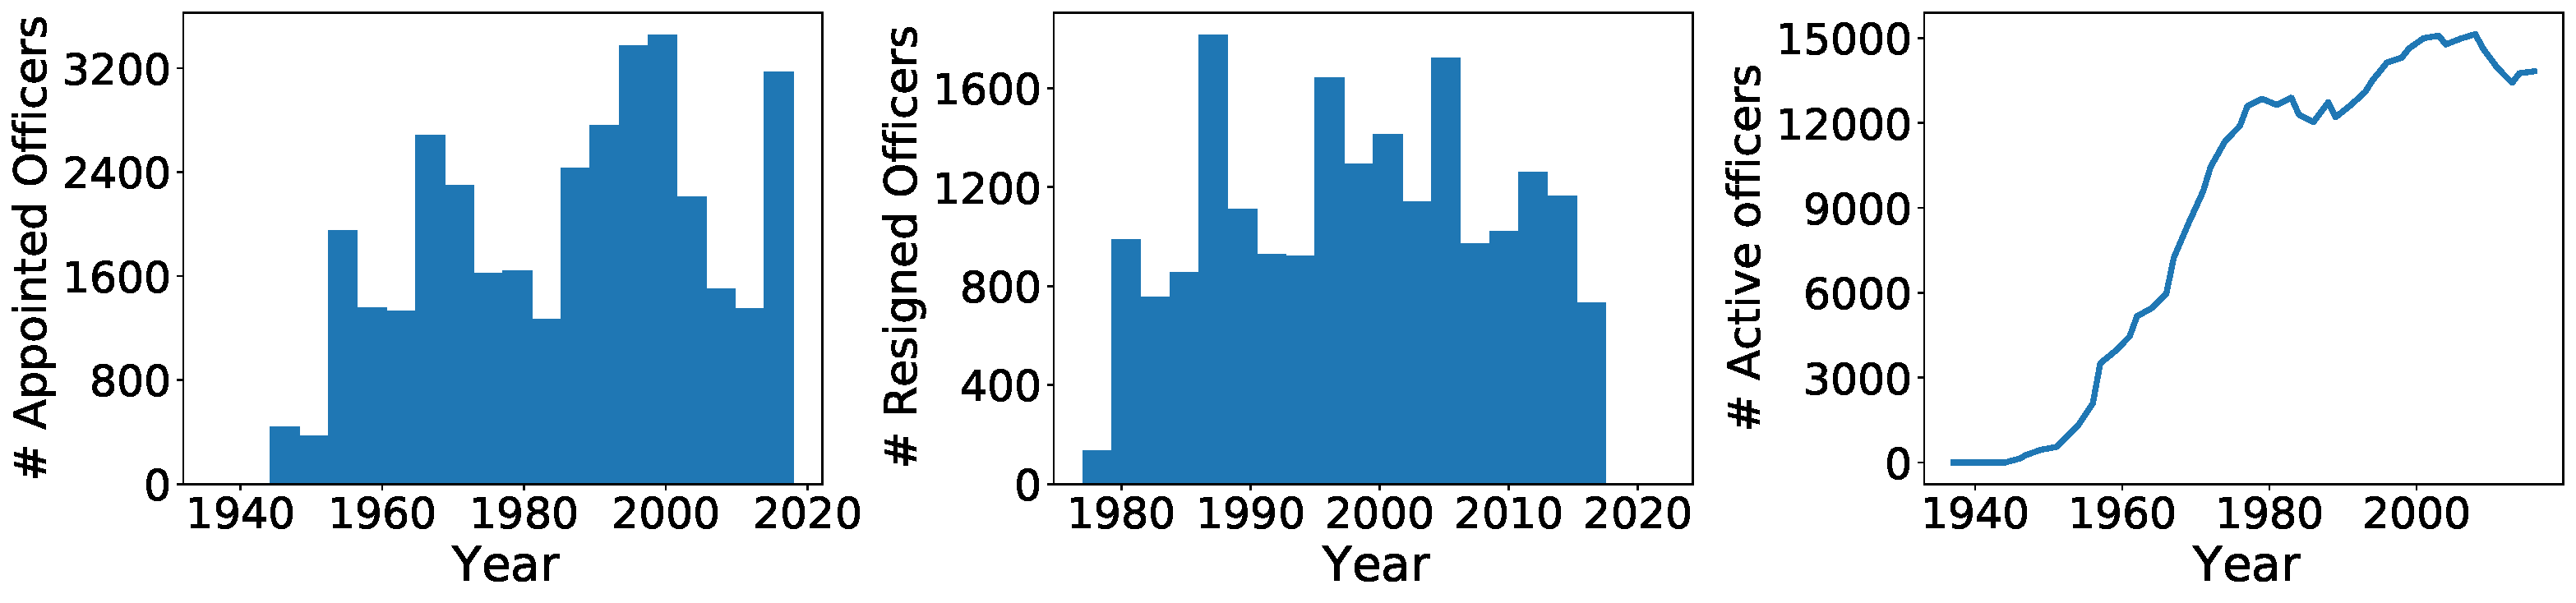
\includegraphics[width=\textwidth]{figs/history} 
	\caption{Historical data from the CPD. The left subplot shows the number of officers' appointments, the central subplot the number of officers' resignations, while the right subplot shows the number of active officers in the database (vertical axis) as a function of time (horizontal axis).} \label{fig:history}
\end{figure}

\begin{table}[h]
\begin{tabular}{l|c|c|c|c|c|c|c|c|c|c|}
\cline{2-3} \cline{5-11}
                                               & \multicolumn{2}{c|}{\textit{\textbf{Gender}}} & \multicolumn{1}{l|}{} & \multicolumn{7}{c|}{\textit{\textbf{CPD Race Category}}}                                                                                                                                                            \\ \cline{2-3} \cline{5-11} 
                                               & \textit{\textbf{M}}   & \textit{\textbf{F}}   &                       & \textit{\textbf{White}} & \textit{\textbf{Black}} & \textit{\textbf{Wh. Hisp.}} & \textit{\textbf{Asian}} & \textit{\textbf{Hisp.}} & \multicolumn{1}{l|}{\textit{\textbf{Am. Ind.}}} & \textit{\textbf{Bl. Hisp.}} \\ \cline{1-3} \cline{5-11} 
\multicolumn{1}{|c|}{\textit{\textbf{All}}}    & 31147                 & 11644                 &                       & 22995                   & 11303                   & 5019                        & 658                     & 348                     & 77                                              & 9                           \\ \cline{1-3} \cline{5-11} 
\multicolumn{1}{|c|}{\textit{\textbf{Active}}} & 13944                 & 8878                  &                       & 9121                    & 6570                    & 3802                        & 542                     & 348                     & 50                                              & 9                           \\ \cline{1-3} \cline{5-11} 
\end{tabular}
\caption{Summary statistics (gender, race) for all officer (first row), as well as for active officers --- those whose resignation date is not before Jan 1st 2019.} \label{tab:stats}
\end{table}

\begin{figure}[h] 
	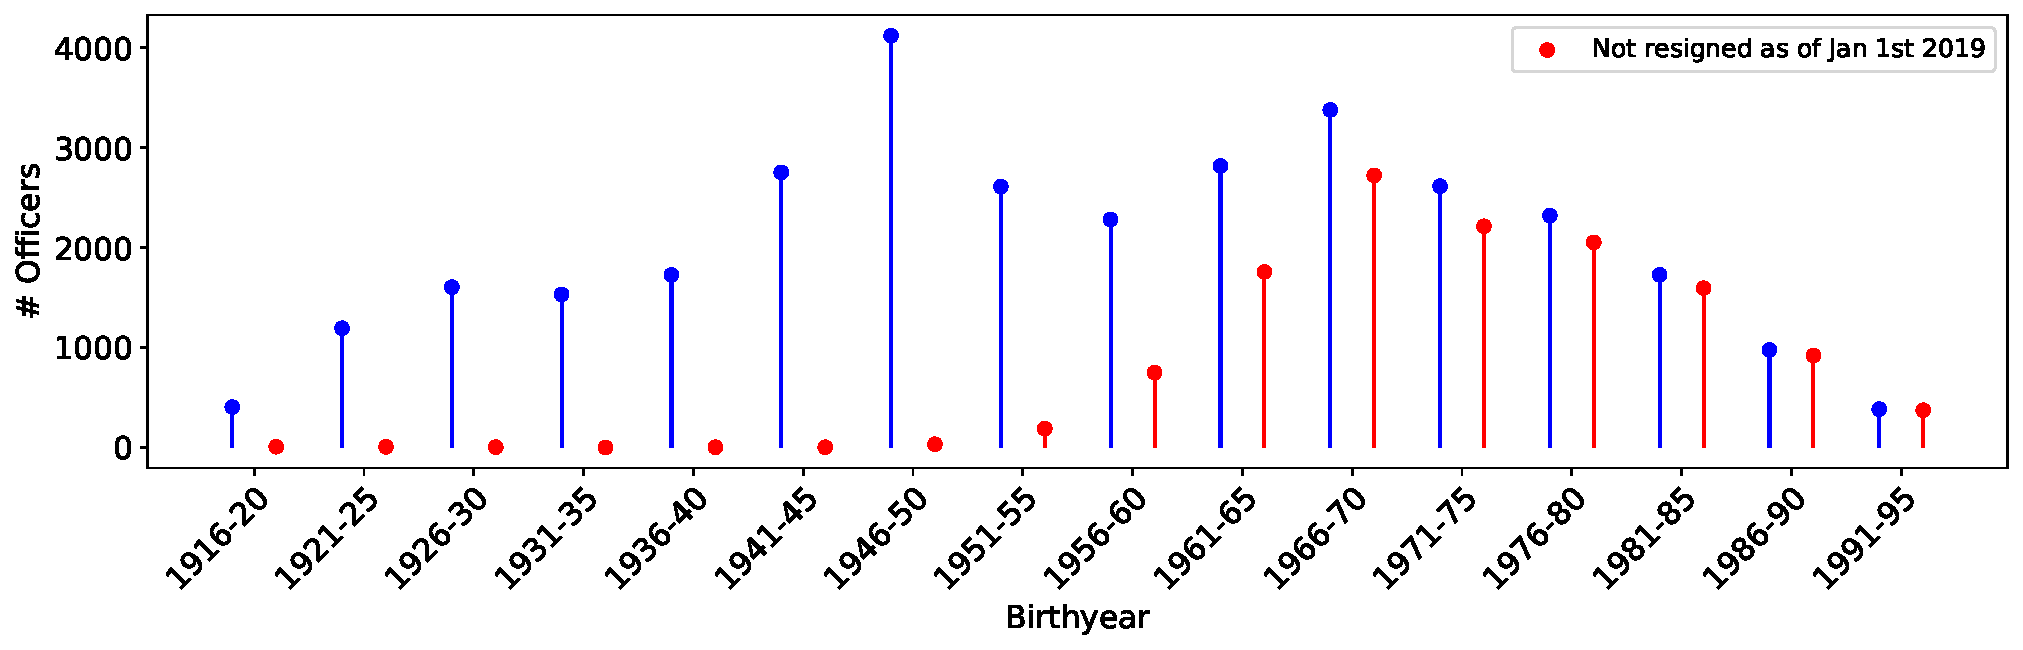
\includegraphics[width=\textwidth]{figs/history_by} 
	\caption{Historical data from the CPD. Birthyears for officers in the CPD dataset: blue dots count all officers, while red count only officers who are ``active'' as of January 1st, 2019.} \label{fig:history_by}
\end{figure}

\subsection{Tactical response reports}

The file \texttt{P0-46360\_main.csv} contains information about tactical response reports, filed as a consequence of  events involving use of force of CPD officers. This dataset contains $9{,}246$ distinct events, as identified by the index ``\texttt{event\_no}'', between January 17th 2004 and April 12th 2016. For each event, the time and location is recorded. Details about the officers involved, as well as the civilian subject are available too. 

\subsection{Salary}

\begin{figure}[h] 
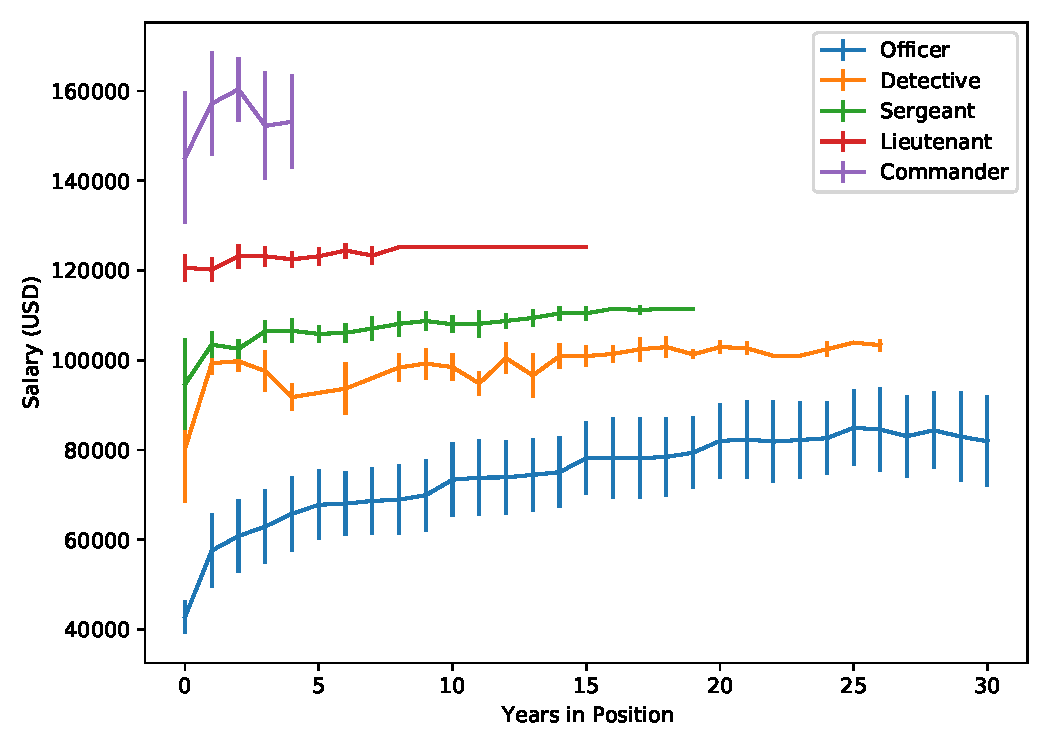
\includegraphics[width=\textwidth]{figs/salary} 
\caption{Historical data from the CPD. Salary versus experience in each
position, years x axis, salary (USD) y axis, for a few of the most common
positions. Lines are means, bars indicate 1 std dev above and below.} \label{fig:salary}
\end{figure}

\begin{figure}[h] 
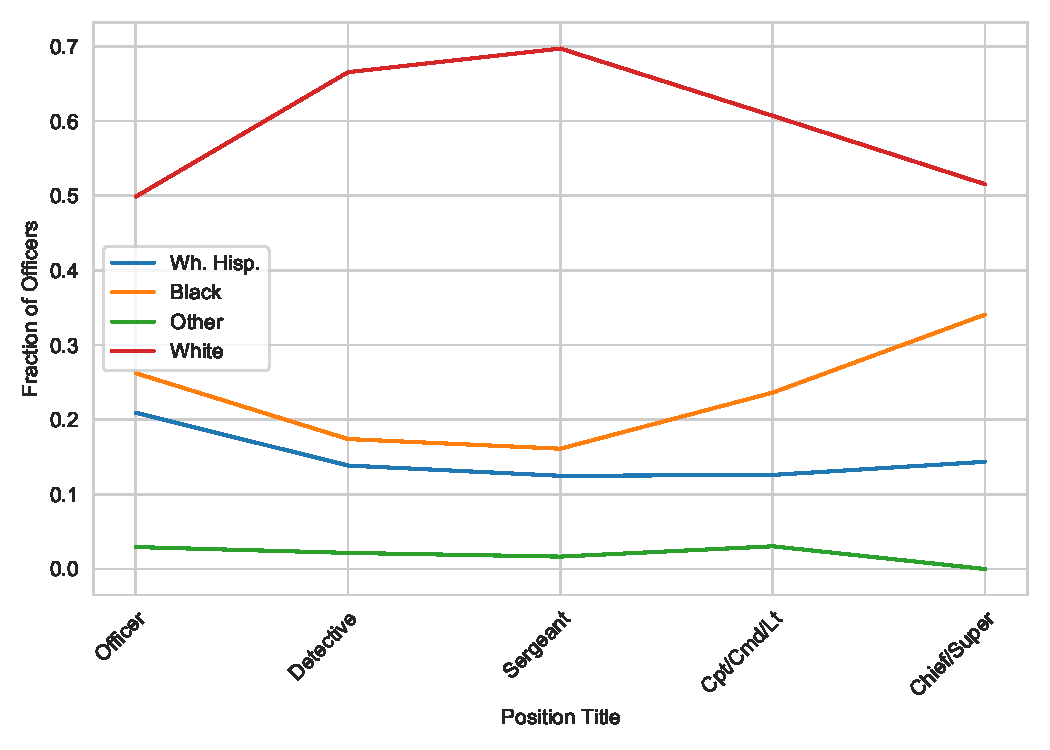
\includegraphics[width=\textwidth]{figs/position_race} 
\caption{Historical data from the CPD. Fraction of officers in representative positions 
per race category.} \label{fig:salary}
\end{figure}

\begin{figure}[h] 
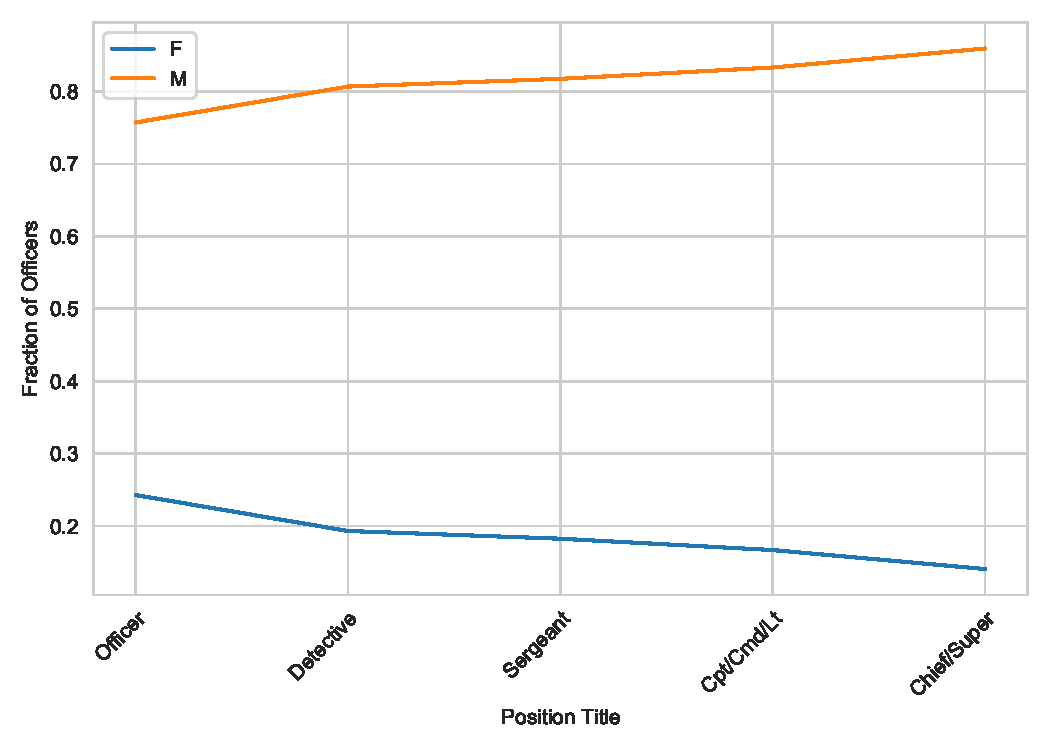
\includegraphics[width=\textwidth]{figs/position_gender} 
\caption{Historical data from the CPD. Fraction of officers in representative positions 
per gender category.} \label{fig:salary}
\end{figure}

\subsection{Awards}

\begin{figure}[h] 
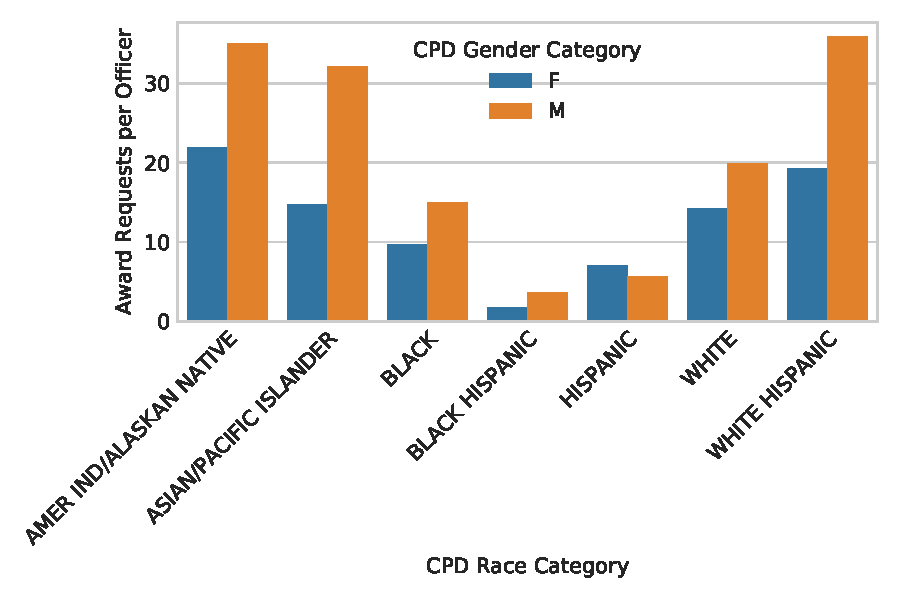
\includegraphics[width=\textwidth]{figs/awards} 
\caption{Historical data from the CPD. Awards per officer vs race for the two cpd gender categories.} \label{fig:awards}
\end{figure}


